\documentclass[12pt]{article}

\input preamble

\title{Principles of Parallel Architecture\\
Synchronization}
\author{Xitong Liu \\
xliu@ece.udel.edu}

\begin{document}

\maketitle

\section{Synchronization Primitives}
\subsection{Description}
The objective of this part is to learn how to write fast synchronization 
primitives. And what are the key characteristics that they expose.

Research what atomic operations can be used on cluster. A few suggestions 
read the file \texttt{/proc/cpuinfo} on cluster, and read the following 
website:

\texttt{http://gcc.gnu.org/onlinedocs/gcc-4.1.2/gcc/Atomic-Builtins.html}

Describe briefly the atomic operations and its syntax.

\subsection{Answer}
These build-in functions were provided by GCC to implement the atomic 
operation on Intel Intanium Processors. All these function will be 
translated to Intel Intanium Processor-specific assembly intrinsics.

There are four groups of functions. The first group were
\begin{verbatim}
type __sync_fetch_and_add (type  *ptr, type value, ...)
type __sync_fetch_and_sub (type *ptr, type value, ...)
type __sync_fetch_and_or (type *ptr, type value, ...)
type __sync_fetch_and_and (type *ptr, type value, ...)
type __sync_fetch_and_xor (type *ptr, type value, ...)
type __sync_fetch_and_nand (type *ptr, type value, ...)
\end{verbatim}
in which the value at \texttt{*ptr} will be fetched first and the associated 
operation (e.g. add, sub, or, and) will be applied. The operands for the
operation are the value at \texttt{*ptr} and passed-in \texttt{value} as 
parameter. The result of the operation will be stored at \texttt{*ptr}. The 
old value at \texttt{*ptr} will be returned then.

The second group were
\begin{verbatim}
type __sync_add_and_fetch (type  *ptr, type value, ...)
type __sync_sub_and_fetch (type *ptr, type value, ...)
type __sync_or_and_fetch (type *ptr, type value, ...)
type __sync_and_and_fetch (type *ptr, type value, ...)
type __sync_xor_and_fetch (type *ptr, type value, ...)
type __sync_nand_and_fetch (type *ptr, type value, ...)
\end{verbatim}
They are basically the same with the first group. The only difference between 
them is that the second group functions apply the operation on the operands 
first, and the new value at \texttt{*ptr} will be returned.

The third group were
\begin{verbatim}
bool __sync_bool_compare_and_swap (type  *ptr, type oldval type newval, ...)
type __sync_val_compare_and_swap (type *ptr, type oldval type newval, ...)
\end{verbatim}
These two function perform an atomic compare and swap. If the current value of 
\texttt{*ptr} is \texttt{oldval}, then write \texttt{newval} into \texttt{*ptr}.

The last group were
\begin{verbatim}
__sync_synchronize (...)
type __sync_lock_test_and_set (type  *ptr, type value, ...)
void __sync_lock_release (type *ptr, ...)
\end{verbatim}
The first function performs a full memory barrier. The last two functions were 
not traditional test-and-set operations, but rather an atomic exchange operation. 
The second function writes value into \texttt{*ptr}, and returns the previous 
contents of \texttt{*ptr} and the third function write the constant 0 to 
\texttt{*ptr}.

\section{Primitive implementation and performance evaluation}
\subsection{Description}
The objective of this part of the homework is to learn how to write 
synchronization operations.

\subsection{Answer}
The source code were placed in directory \texttt{my\_sync}.

The mutex was defined as below:
\begin{verbatim}
typedef struct _my_mutex_t{
  volatile int lock;
}my_mutex_t;

#define LOCKED 1
#define FREE   0
#define LOCK_WAIT_INTERVAL 100
\end{verbatim}
and the implementation for lock and unlock operation were
\begin{verbatim}
void my_mutex_lock(my_mutex_t * p){
  // wait for the lock to be freed, lock it then
  while(!__sync_bool_compare_and_swap(&(p->lock), FREE, LOCKED)){
    usleep(LOCK_WAIT_INTERVAL);
  }
}
void my_mutex_unlock(my_mutex_t * p){
  __sync_lock_test_and_set(&(p->lock), FREE);
}
\end{verbatim}
The the lock operation, since \texttt{\_\_sync\_bool\_compare\_and\_swap} 
will check the value \texttt{p->lock} is equal with \texttt{FREE}. 
If the mutex if locked, \texttt{p->lock} will be \texttt{LOCKED} and
\texttt{\_\_sync\_bool\_compare\_and\_swap} will return false with nothing
changed. So the current thread will wait for \texttt{LOCK\_WAIT\_INTERVAL}
microseconds and check it again. If the lock is freed, \texttt{p->lock} 
will be \texttt{FREE} and \texttt{\_\_sync\_bool\_compare\_and\_swap} will 
set it back to \texttt{LOCKED} and return true. Then the function
\texttt{my\_mutex\_lock} will return and the current thread will be the 
owner of the lock. Since the lock and unlock were implemented in atomic 
operation, it's guaranteed that \texttt{p->lock} will be accessed by only one
thread at any times. 

The barrier was defined as below:
\begin{verbatim}
typedef struct _my_barrier_t{
  volatile int sense;
  volatile int num_p;
  volatile int cur_p;
  volatile int occupied;
  volatile my_mutex_t lock;
}my_barrier_t;

#define BARRIER_NA       0
#define BARRIER_AVAIL    1
#define BARRIER_FREE     0
#define BARRIER_OCCUPIED 1
#define BARRIER_WAIT_INTERVAL 100
\end{verbatim}
and the wait operation was defined as
\begin{verbatim}
void my_barrier_wait(my_barrier_t * p){
  while(BARRIER_OCCUPIED == p->occupied){
    usleep(BARRIER_WAIT_INTERVAL);
  }

  // lock it first
  my_mutex_lock((my_mutex_t*)&(p->lock));
  // Atomically add the the counter of current peers
  ++(p->cur_p);
  
  if(p->cur_p == p->num_p){
    // yes, notify other peers
    p->sense = BARRIER_AVAIL;
    p->occupied = BARRIER_OCCUPIED;
  }else{
    p->sense = BARRIER_NA;
  }
  // unlock it then
  my_mutex_unlock((my_mutex_t*)&(p->lock));

  // else, wait for other peers
  while(BARRIER_NA == p->sense){
    usleep(BARRIER_WAIT_INTERVAL);
  }
 
  my_mutex_lock((my_mutex_t*)&(p->lock));
  --(p->cur_p);
  if(0 == p->cur_p){
    p->occupied = BARRIER_FREE;
  }
  my_mutex_unlock((my_mutex_t*)&(p->lock));
}
\end{verbatim}
These is a mutex lock in one barrier to ensure the increase operation for 
\texttt{p->cur\_p} and compare operation between \texttt{p->cur\_p} and 
\texttt{p->num\_p} is applied in atomic manner. When the last thread reached
the barrier, \texttt{p->sense} will be marked to notify other peers to leave
the barrier. \texttt{p->occupied} will also be marked so all the threads will 
not run into another barrier. Instead they will wait before the next barrier 
until all the thread have leave the previous barrier and \texttt{p->occupied} 
is cleared. Without \texttt{p->occupied} it will got stuck into infinite waiting
state if some thread have not leaved the previous barrier while other threads
have already run into a new barrier.

The result were shown as below:
\begin{verbatim}
Running with P=8 N=3500
Now running [Barrier Correctness]
++++++++++
Tests passed: 10 of 10. Average Time = 13.092589 (sec)
Now running [Barrier Performance]
++++++++++
Tests passed: 10 of 10. Average Time = 10.881422 (sec)
Now running [Lock Correctness]
++++++++++
Tests passed: 10 of 10. Average Time = 0.518503 (sec)
Now running [Lock Performance]
++++++++++
Tests passed: 10 of 10. Average Time = 0.222413 (sec)
Running with P=16 N=3500
Now running [Barrier Correctness]
++++++++++
Tests passed: 10 of 10. Average Time = 13.307263 (sec)
Now running [Barrier Performance]
++++++++++
Tests passed: 10 of 10. Average Time = 11.126159 (sec)
Now running [Lock Correctness]
++++++++++
Tests passed: 10 of 10. Average Time = 1.047272 (sec)
Now running [Lock Performance]
++++++++++
Tests passed: 10 of 10. Average Time = 0.405896 (sec)
\end{verbatim}



\end{document}

\begin{comment}
\begin{figure}[h!]
	\begin{center}
		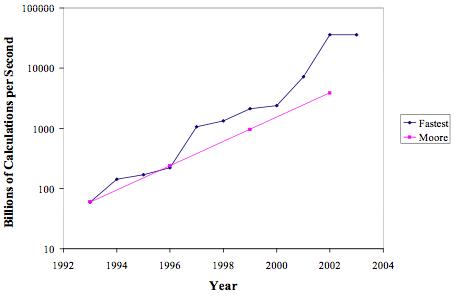
\includegraphics[width=0.7\textwidth, angle=0]{fatest.png}
		\caption{\label{fig:fatest}Fatest SuperComputer in the world}
	\end{center}
\end{figure}
\end{comment}